\documentclass{IEEEtran}
%% PACKAGES %%

\usepackage{amsmath, amsfonts, amssymb, amsthm}
\usepackage{braket}
\usepackage{listings}
\usepackage{geometry}
\usepackage{xcolor}
\usepackage{textcomp}
\usepackage{graphicx}
\usepackage{fancyhdr}
\usepackage{sourcecodepro}
\usepackage{multirow}

%%%%%%%%%%%%%%

\hbadness = 99999 % remove annoying warning

\graphicspath{{./images}}

% Title Stuff
\title{ECE296 PLC Lab 0 - Logic Gates}
\author{Chase A. Lotito, \textit{SIUC Undergraduate}}
\date{}

\begin{document}

\maketitle % Makes the title

\section{Introduction} 
% (Brief description of how the lab was setup and the steps you took while completing the tasks given)

This experiment was an introduction to the programmable logic controller (PLC). The particular PLC being the Allen-Bradley MicroLogix 1100, which we can program with ladder logic in \textit{RSLogix}. 

Using the toggle switches as inputs (SW1 and SW2), the goal is to recreate the functionality of 2-bit AND, OR, and XOR logic gates. They should follow these equations if \(A = SW1\) and \(B = SW2\):

\begin{align}\label{eq:logicgates}
    \text{AND} &: A \cdot B \\
    \text{OR} &: A + B \\
    \text{XOR} &: A \cdot \bar{B} + \bar{A} \cdot B
\end{align}

The blue light represents the output for AND, the green light for OR, and the yellow light for XOR.

\section{Assessment of Design}
% (How did it work in the end? Any problems or missteps along the way? Explain key aspects of design. Attach images of working design.)

The specific ladder logic used can be seen in \textit{Appendix A}. 

In order to check if a switch is "on" or "off", we need to first designate the I/O as normally open (NO) or normally closed (NC). For NO, if "off" we get 0, and if "on" we get 1. For NC, if "off" we get 1, and if "on" we get 0. Essentially, NO preserves the state of the switch, and NC inverts the state of the switch.

A series combination of NO and or NC contacts requires both to be 1 for continuity, so that acts as an AND operation. A parallel combination of NO and or NC contacts only requires a single contact to be 1 for continuity, so that acts as an OR operation.

Figure \ref{fig:ladderlogic} shows these principles applied to Eq. \ref{eq:logicgates}.

%\begin{figure}[!ht] 
%    \centering
%    \includegraphics[width = 7cm]{}
%    \caption{}
%    \label{fig:}
%\end{figure}

\section{Conclusion}
% (What did you learn during this lab? Final thoughts or findings? Did you meet the objectives? Answer any questions given in the lab manual here.)

\section*{Appendix A: Ladder Logic}

\begin{figure}[!ht] 
    \centering
    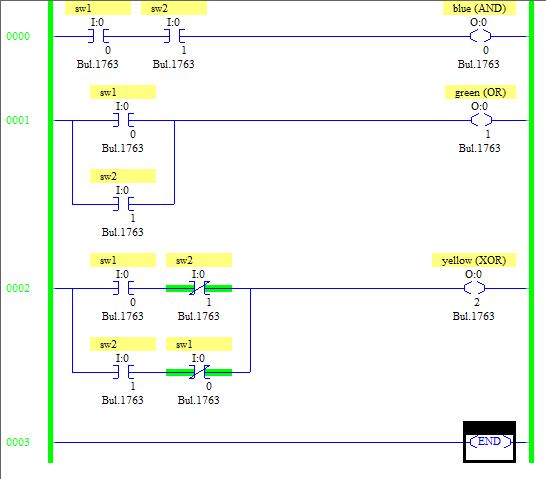
\includegraphics[width = 7.3cm]{ladderlogic.png}
    \caption{Ladder Logic for Logic Gates}
    \label{fig:ladderlogic}
\end{figure}

\end{document}
